\section{Background}\label{sec:background}

\subsection{Sensor database systems}
%/* Review the system (Towards a sensor database is a good source \& tinyDB arch.). With an example of a query and platform/application. */
Sensor networks are being widely deployed for measurement, detection and surveillance applications.  Related work to data processing in a wireless sensor network is TinyDB, a query processing system for extracting information from a sensor network. TinyDB provides a SQL like interface, for each input request it collects data from the nodes, filters it and sends the aggregated result to a PC via power efficient network processing algorithm. Queried data consists of sensor attributes (e.g., location) as well as sensor data. A typical monitoring scenario involves aggregate queries or correlation queries. In order to optimize the system's  performance, result of these queries are partially aggregated at each intermediate node. In our system we have implemented an interface to query on the properties such as the sensor temperature and further grouped the results on the basis of floor numbers.

\begin{figure}[t]
\centering
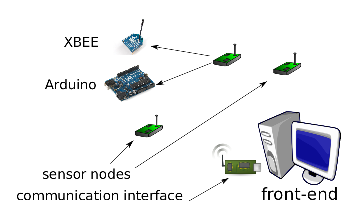
\includegraphics[scale=1.2]{figures/topology.eps}
\caption{Components used in the prototype}
\label{fig:topology}
\end{figure}

\subsection{Prototype infrastructure}
%/* speak here about arduino, XBee, ZigBee protocol, and 802.15.4 */
A depiction of our prototype is supplied in Figure~\ref{fig:topology}. It consists of a front-end that receives external requests and delivers readings for outside users. The back-end is a collection of sensor nodes consisting of a micro-controller and a wireless module. A detailed description of used components follows:
\begin{itemize}
\item{\emph{Arduino}: Arduino is a micro-controller capable of sensing the environment by receiving the input from sensors in its surroundings. The micro-controller on the board is programmed using the Arduino programming language (based on C/C++ library) and the Arduino development environment (based on Processing). In Arduino the connectors are exposed in such a way that allows CPU boards to be connected to a variety of interchangeable add-on modules. In our experiments we use Arduino Uno boards.}
\item{\emph{XBEE}: XBee is a radio module based on IEEE 802.15.4 networking protocol providing wireless end-point connectivity to devices.  It is designed for high-throughput application which require low latency and predictable communication timing. AT commands are used to control the radio settings. They can operate either in a transparent data mode or in a packet based (API) mode. In the transparent mode data coming into the DIN (Data IN) pin gets directly transmitted to the intended receiving radios without any modification. Incoming packets can either be directly addressed to one target or broadcast to multiple targets. This mode is primarily used in instances where an existing protocol cannot tolerate changes to the data format. We use XBee series 2 modules.}
\item{\emph{ZigBee}: ZigBee is a specification for a suite of high level communication protocols using small, low-power digital radios based on an IEEE 802 standard for Personal Area Network (PAN). ZigBee builds upon the physical layer and medium access control defined in IEEE standard 802.15.4 (2003 version) for low-rate wireless PANs.  It is targeted at radio-frequency (RF) applications that require a low data rate, long battery life, and secure networking. ZigBee data rate varies from 20 kbps to 900 kbps but 250 kbps is best suited for periodic or intermittent data or a single signal transmission from a sensor or input device. The current ZigBee protocol supports beacon and non-beacon enabled networks.  In non-beacon-enabled networks, an unslotted CSMA/CA channel access mechanism is used and receivers always remains active. In beacon enabled mode, ZigBee router transmit periodic beacons to confirm their presence to other network nodes. Nodes may sleep between beacons to extend their battery life. In our experiments we operate in non-beacon mode. There are three different types of Zigbee devices: 
\begin{itemize}
\item{\emph{ZigBee Coordinator (ZC)}: it forms the root of the network tree and might bridge to other networks. There is exactly one ZC per network. }
\item{\emph{ZigBee Router (ZR)}: it can run an application and can also act as an intermediate router. }
\item{\emph{ZigBee End Device (ZED)}: It has the capability to talk to the parent node. It cannot relay data from other devices. This relationship allows the node to be asleep a significant amount of the time thereby giving long battery life.}
\end{itemize}
}
\end{itemize}
